% arara: pdflatex: {files: [MathSACpr2014]}
\chapter{Other  Curricular Issues}
\section[Distance education]{To what degree are courses offered in a Distance modality (on-line, hybrid, interactive television, etc)? For courses offered both via DL and on-campus, are there differences in student success? (Contact the Office of Institutional Effectiveness , either Laura Massey or Rob Vergun,  for course-level data). If so, how are you, or will you address these differences? What significant revelations, concerns or questions arise in the area of DL delivery?}

\subsection{Presence of DL offerings}
The Math SAC offers Distance Learning (DL) courses in on-line, hybrid, and interactive television (ITV) modalities.  We strive to make our DL course experience simulate the face-to-face course experience with respect to instructor presence, feedback, and assessment. We use discussion boards to simulate the classroom learning environment, and an array of online homework platforms to assess and prepare our students effectively. A Math SAC DL standing committee is charged with discussing the structure of our current DL courses, as well as developing and maintaining current DL best practices and standards.

All of our pre-college level math courses (except a calculator skills course) have a DL offering, as do most of our lower-division collegiate courses.  Courses that are not offered using a distance modality fall into two categories: those on the high end of our collegiate courses, and specialty courses with low enrollments. See \cref{tab:sec3:DLofferings}.

\begin{table}
\caption{Course Offerings through Distance Learning}\label{tab:sec3:DLofferings}
\centering
\begin{tabular}{p{1in}p{1in}p{1in}}
\toprule
Offered as DL & Not offered  DL upper division & Not offered  DL specialty\\
\midrule
020, 030, 060, 065, 070, 084, 095, 111, 112, 241, 243, 244&
251, 252, 253, 254, 256, 261&
015, 25C, 26C, 061, 062, 063, 093, 105, 211, 212, 213\\
\bottomrule
\end{tabular}
\end{table}

Approximately 14.1\% of PCC math enrollments were into a DL class during the academic year of 2012/13 compared to only 9.1\% in the 2007/08 academic year. This percentage increase is coupled with a general enrollment surge over the past five years, and the number of DL enrollments has grown by over 150\% in this time period. \Cref{tab:sec3:F2FandDLenrollments} shows student enrollment in face-to-face courses compared to online courses over six academic years.

\begin{figure}[!htb]
    \begin{minipage}{.5\textwidth}
          %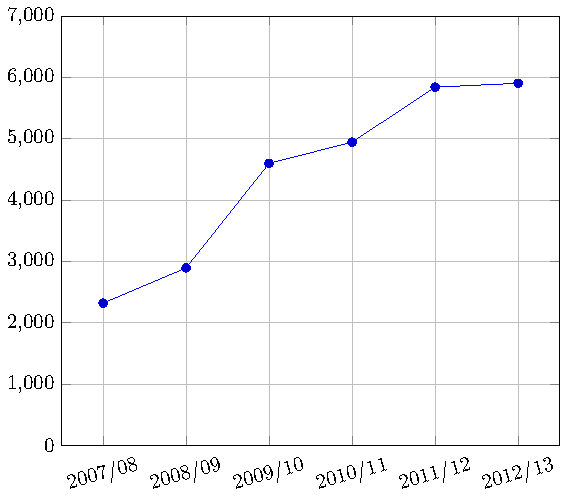
\includegraphics[width=\textwidth]{graphics/enrollmentInDL.pdf}
          % arara: pdflatex
% !arara: indent: {overwrite: yes}
\documentclass{standalone}
% Caption: Enrollment in DL
% 2007/08-2012/13

\usepackage{pgfplots}
\usepackage{pgfplotstable}
\pgfplotsset{compat=newest}


\begin{document}

% http://tex.stackexchange.com/questions/128468/problems-with-pgfplotstableread-and-relative-paths
\IfStandalone{
	\newcommand{\fromRoot}[1]{../data/#1}
	}{
	\newcommand{\fromRoot}[1]{./data/#1}
}

% need to have the read command in the main document, otherwise it will 
% be ignored when used with standalone
\pgfplotstableread[col sep=comma]{\fromRoot{ProcessedGradesData.csv}}\enrollmentdata

\begin{tikzpicture}
	\begin{axis}[
			%ybar,
			symbolic x coords={2007/08, 2008/09, 2009/10, 2010/11, 2011/12, 2012/13, NaN},
			xtick=data,
			minor ytick={1000,2000,...,7000},
			enlarge x limits,
			%scale only axis,       
			grid = both,
			ymin=0,ymax=7000,
			scaled ticks=false, 
			tick label style={/pgf/number format/fixed},
			legend pos=outer north east,
			restrict x to domain=0:5,
			x tick label style={rotate=25},
			width=\textwidth,
		]
		\addplot table[x=AY,y=DL_Enrollments]{\enrollmentdata};
		%\legend{DL}
	\end{axis}
\end{tikzpicture}
\end{document}

          \caption{Enrollments in DL}
    \end{minipage}%
    \begin{minipage}{.5\textwidth}
          %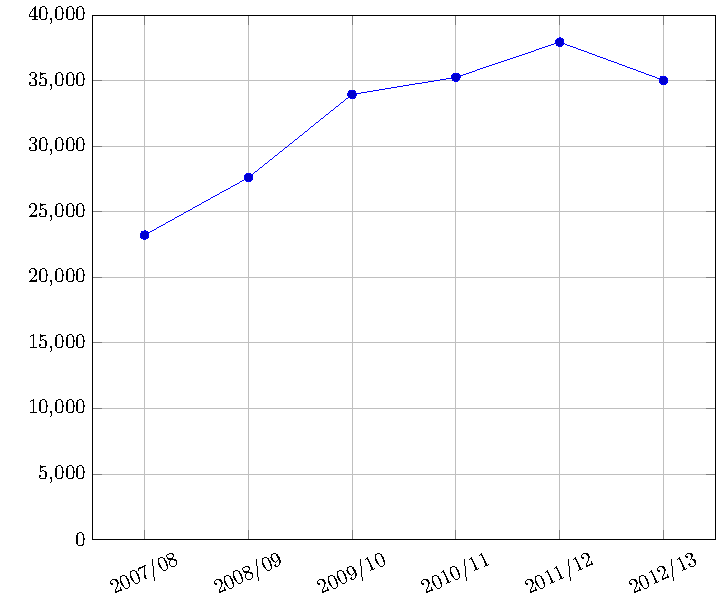
\includegraphics[width=\textwidth]{graphics/enrollmentInF2F.pdf}
          % arara: pdflatex
% !arara: indent: {overwrite: yes}
\documentclass{standalone}
% Caption: Enrollment in F2F
% 2007/08-2012/13

\usepackage{pgfplots}
\usepackage{pgfplotstable}
\pgfplotsset{compat=newest}

\pgfplotstableread[col sep=comma]{../data/ProcessedGradesData.csv}\enrollmentdata

\begin{document}

\begin{tikzpicture}
	\begin{axis}[
			%ybar,
			symbolic x coords={2007/08, 2008/09, 2009/10, 2010/11, 2011/12, 2012/13, NaN},
			xtick=data,
			%minor ytick={1000,5000,...,40000},
			enlarge x limits,
			scale only axis,       
			grid = both,
			ymin=0,ymax=40000,
			scaled ticks=false, 
			tick label style={/pgf/number format/fixed},
			legend pos=outer north east,
			restrict x to domain=0:5,
			x tick label style={rotate=15},
		]
		\addplot table[x=AY,y=F2F_Enrollments]{\enrollmentdata};
		%\legend{DL}
	\end{axis}
\end{tikzpicture}
\end{document}

          \caption{Enrollments in F2F}
    \end{minipage}
         \captionof{table}{Table Caption goes here}\label{tab:sec3:F2FandDLenrollments}
\end{figure}

\fixthis{is the above table caption appropriate?}

As enrollment demand for DL math courses has increased, we have increased the number of sections that we offer and trained more interested faculty in managing DL courses.  Between the academic years of 2003/04 and 2007/08, the annual number of sections offered increased from 51 to 87.  In the 2012/13 academic year, we offered 185 DL sections.   The resulting increase in sections offers access to students that can succeed in this modality and need this option due to outside constraints such as work and family.


\subsection{Success Rates in DL courses}
Pass rates in DL courses are significantly lower than those for their face-to-face counterparts. We recognize that students need a certain level of self-discipline, better study skills, and comfort engaging with technology to succeed in a DL course. However we currently have no method for screening which students are less likely to succeed using a distance modality.  \Cref{fig:sec3:F2FandDLpassRates} shows the difference in pass rates between the DL courses that we offer and their face-to-face counterparts.  It is clear that, in the six academic years shown, the passing rates are generally decreasing regardless of delivery mode.  We hypothesize that this overall trend is mostly the result of the economic collapse of 2008 which led to increased enrollment and changes in our student demographics (REF to diversity section?).  But the pass rates in DL courses are as much as 30\% lower than in face-to-face counterparts and this large discrepancy needs to be addressed.

\begin{figure}[!htb]
  \begin{widepage}
    \begin{subfigure}{.3\textwidth}
          %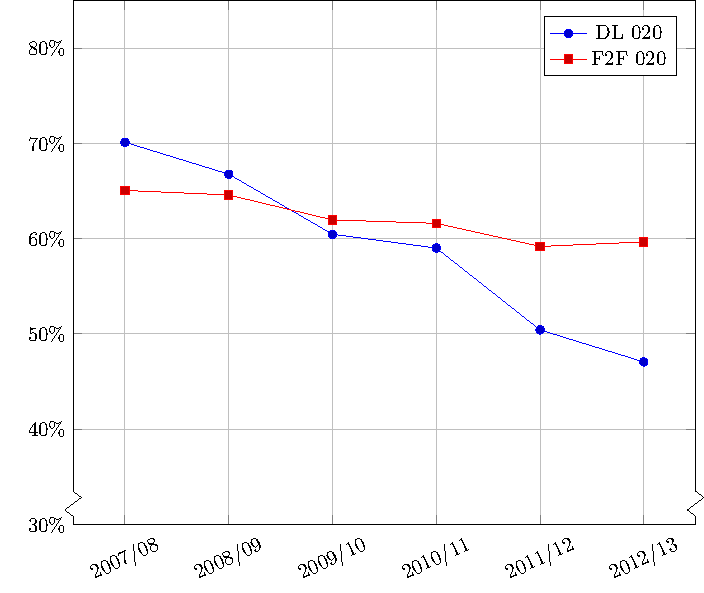
\includegraphics[width=\textwidth]{graphics/passRatesByModality020.pdf}
          % arara: pdflatex
% !arara: indent: {overwrite: yes}
\documentclass{standalone}
% Caption: Enrollment in DL
% 2007/08-2012/13

\usepackage{pgfplots}
\usepackage{pgfplotstable}
\pgfplotsset{compat=newest}

\pgfplotstableread[col sep=comma]{../data/ProcessedGradesData.csv}\enrollmentdata

\begin{document}

\begin{tikzpicture}
	\begin{axis}[
			%ybar,
			symbolic x coords={2007/08, 2008/09, 2009/10, 2010/11, 2011/12, 2012/13, NaN},
			xtick=data,
			%minor ytick={1000,2000,...,7000},
			enlarge x limits,
			scale only axis,       
			grid = both,
			ymin=0.3,ymax=0.85,
			axis y discontinuity=crunch,
			scaled ticks=false, 
			tick label style={/pgf/number format/fixed},
			legend pos=outer north east,
			restrict x to domain=0:5,
			x tick label style={rotate=15},
		]
		\addplot table[x=AY,y=020_DL_Pass_Rate]{\enrollmentdata};
		\addplot table[x=AY,y=020_F2F_Pass_Rate]{\enrollmentdata};
		\legend{DL 020, F2F 020}
	\end{axis}
\end{tikzpicture}
\end{document}

          \captionof{figure}{MTH 20}
    \end{subfigure}%
    \begin{subfigure}{.3\textwidth}
    %      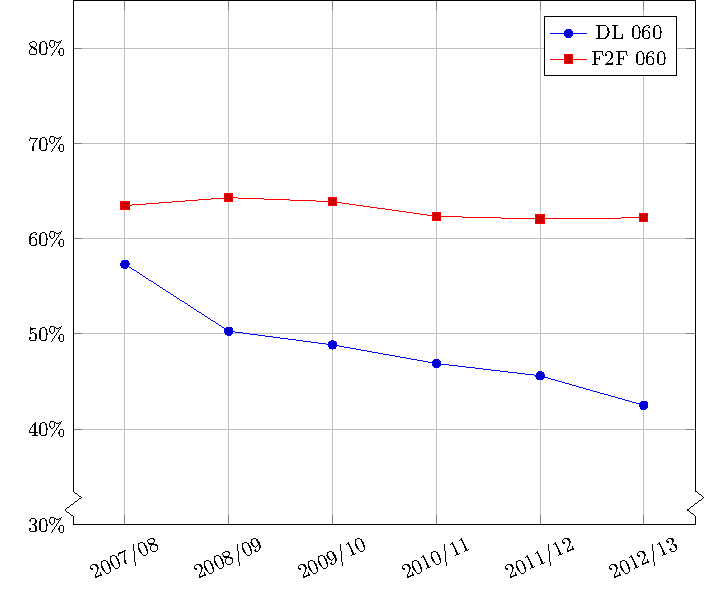
\includegraphics[width=\textwidth]{graphics/passRatesByModality060.pdf}
          % arara: pdflatex
% !arara: indent: {overwrite: yes}
\documentclass{standalone}
% Caption: Enrollment in DL
% 2007/08-2012/13

\usepackage{pgfplots}
\usepackage{pgfplotstable}
\pgfplotsset{compat=newest}

\pgfplotstableread[col sep=comma]{../data/ProcessedGradesData.csv}\enrollmentdata

\begin{document}

\begin{tikzpicture}
	\begin{axis}[
			%ybar,
			symbolic x coords={2007/08, 2008/09, 2009/10, 2010/11, 2011/12, 2012/13, NaN},
			xtick=data,
			%minor ytick={1000,2000,...,7000},
			enlarge x limits,
			scale only axis,       
			grid = both,
			ymin=0.3,ymax=0.85,
			axis y discontinuity=crunch,
			scaled ticks=false, 
			tick label style={/pgf/number format/fixed},
			legend pos=outer north east,
			restrict x to domain=0:5,
			x tick label style={rotate=15},
		]
		\addplot table[x=AY,y=060_DL_Pass_Rate]{\enrollmentdata};
		\addplot table[x=AY,y=060_F2F_Pass_Rate]{\enrollmentdata};
		\legend{DL 060, F2F 060}
	\end{axis}
\end{tikzpicture}
\end{document}

          \captionof{figure}{MTH 60}
    \end{subfigure}%
    \begin{subfigure}{.3\textwidth}
          %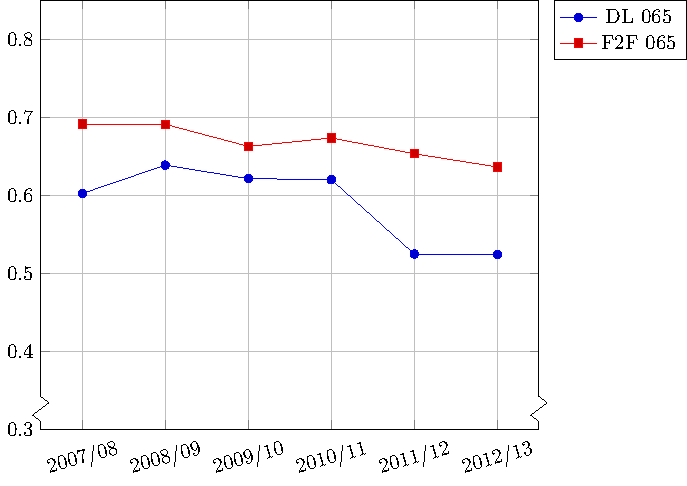
\includegraphics[width=\textwidth]{graphics/passRatesByModality065.pdf}
          % arara: pdflatex
% !arara: indent: {overwrite: yes}
\documentclass{standalone}
% Caption: Enrollment in DL
% 2007/08-2012/13

\usepackage{pgfplots}
\usepackage{pgfplotstable}
\pgfplotsset{compat=newest}


\begin{document}

% http://tex.stackexchange.com/questions/128468/problems-with-pgfplotstableread-and-relative-paths
\IfStandalone{
	\newcommand{\fromRoot}[1]{../data/#1}
	}{
	\newcommand{\fromRoot}[1]{./data/#1}
}
\pgfplotstableread[col sep=comma]{\fromRoot{ProcessedGradesData.csv}}\enrollmentdata

\begin{tikzpicture}
	\begin{axis}[
			%ybar,
			symbolic x coords={2007/08, 2008/09, 2009/10, 2010/11, 2011/12, 2012/13, NaN},
			xtick=data,
			%minor ytick={1000,2000,...,7000},
			enlarge x limits,
			%scale only axis,       
			grid = both,
			ymin=0.3,ymax=0.85,
			axis y discontinuity=crunch,
			scaled ticks=false, 
			tick label style={/pgf/number format/fixed},
			legend pos=south west,
			restrict x to domain=0:5,
			x tick label style={rotate=25},
            width=\textwidth,
		]
		\addplot table[x=AY,y=065_DL_Pass_Rate]{\enrollmentdata};
		\addplot table[x=AY,y=065_F2F_Pass_Rate]{\enrollmentdata};
		\legend{DL 065, F2F 065}
	\end{axis}
\end{tikzpicture}
\end{document}

          \captionof{figure}{MTH 65}
    \end{subfigure}

    \begin{subfigure}{.3\textwidth}
          %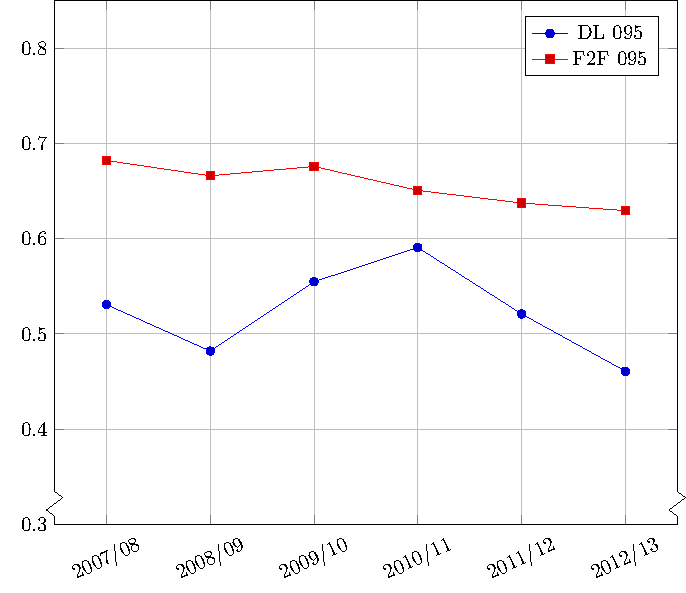
\includegraphics[width=\textwidth]{graphics/passRatesByModality095.pdf}
          % arara: pdflatex
% !arara: indent: {overwrite: yes}
\documentclass{standalone}
% Caption: Enrollment in DL
% 2007/08-2012/13

\usepackage{pgfplots}
\usepackage{pgfplotstable}
\pgfplotsset{compat=newest}


\begin{document}
% http://tex.stackexchange.com/questions/128468/problems-with-pgfplotstableread-and-relative-paths
\IfStandalone{
	\newcommand{\fromRoot}[1]{../data/#1}
	}{
	\newcommand{\fromRoot}[1]{./data/#1}
}
\pgfplotstableread[col sep=comma]{\fromRoot{ProcessedGradesData.csv}}\enrollmentdata

\begin{tikzpicture}
	\begin{axis}[
			%ybar,
			symbolic x coords={2007/08, 2008/09, 2009/10, 2010/11, 2011/12, 2012/13, NaN},
			xtick=data,
			%minor ytick={1000,2000,...,7000},
			enlarge x limits,
			%scale only axis,       
			grid = both,
			ymin=0.3,ymax=0.85,
			axis y discontinuity=crunch,
			scaled ticks=false, 
			tick label style={/pgf/number format/fixed},
			legend pos=north east,
			restrict x to domain=0:5,
			x tick label style={rotate=25},
            width=\textwidth,
		]
		\addplot table[x=AY,y=095_DL_Pass_Rate]{\enrollmentdata};
		\addplot table[x=AY,y=095_F2F_Pass_Rate]{\enrollmentdata};
		\legend{DL 095, F2F 095}
	\end{axis}
\end{tikzpicture}
\end{document}

          \captionof{figure}{MTH 95}
    \end{subfigure}%
    \begin{subfigure}{.3\textwidth}
          %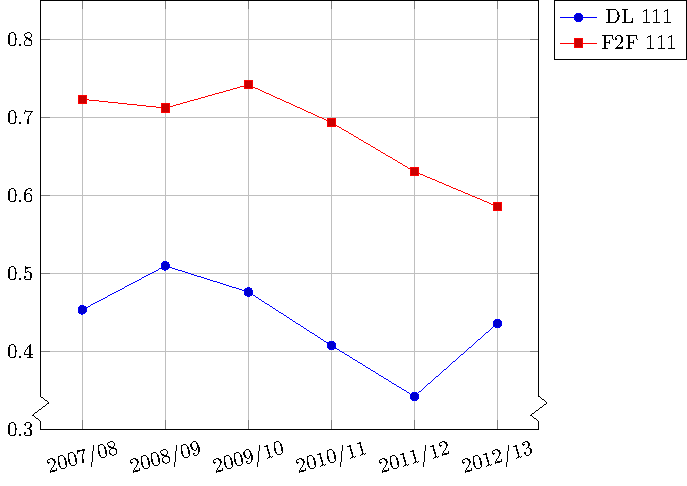
\includegraphics[width=\textwidth]{graphics/passRatesByModality111.pdf}
          % arara: pdflatex
% !arara: indent: {overwrite: yes}
\documentclass{standalone}
% Caption: Enrollment in DL
% 2007/08-2012/13

\usepackage{pgfplots}
\usepackage{pgfplotstable}
\pgfplotsset{compat=newest}

\pgfplotstableread[col sep=comma]{../data/ProcessedGradesData.csv}\enrollmentdata

\begin{document}

\begin{tikzpicture}
	\begin{axis}[
			%ybar,
			symbolic x coords={2007/08, 2008/09, 2009/10, 2010/11, 2011/12, 2012/13, NaN},
			xtick=data,
			%minor ytick={1000,2000,...,7000},
			enlarge x limits,
			scale only axis,       
			grid = both,
			ymin=0.3,ymax=0.85,
			axis y discontinuity=crunch,
			scaled ticks=false, 
			tick label style={/pgf/number format/fixed},
			legend pos=outer north east,
			restrict x to domain=0:5,
			x tick label style={rotate=15},
		]
		\addplot table[x=AY,y=111_DL_Pass_Rate]{\enrollmentdata};
		\addplot table[x=AY,y=111_F2F_Pass_Rate]{\enrollmentdata};
		\legend{DL 111, F2F 111}
	\end{axis}
\end{tikzpicture}
\end{document}

          \captionof{figure}{MTH 111}
    \end{subfigure}%
    \begin{subfigure}{.3\textwidth}
          %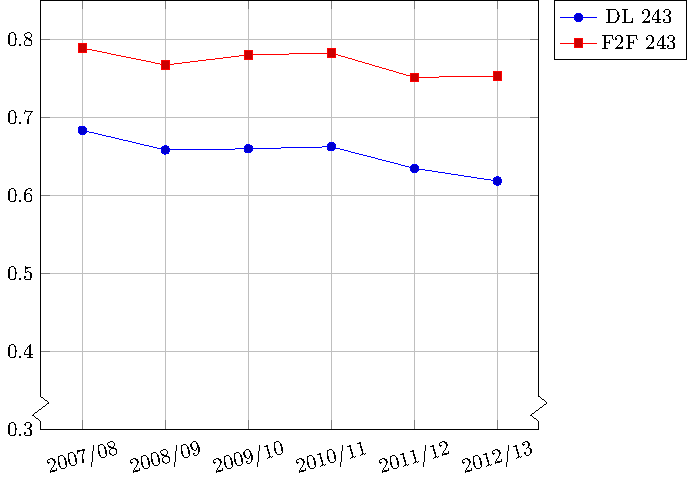
\includegraphics[width=\textwidth]{graphics/passRatesByModality243.pdf}
          % arara: pdflatex
% !arara: indent: {overwrite: yes}
\documentclass{standalone}
% Caption: Enrollment in DL
% 2007/08-2012/13

\usepackage{pgfplots}
\usepackage{pgfplotstable}
\pgfplotsset{compat=newest}

\pgfplotstableread[col sep=comma]{../data/ProcessedGradesData.csv}\enrollmentdata

\begin{document}

\begin{tikzpicture}
	\begin{axis}[
			%ybar,
			symbolic x coords={2007/08, 2008/09, 2009/10, 2010/11, 2011/12, 2012/13, NaN},
			xtick=data,
			%minor ytick={1000,2000,...,7000},
			enlarge x limits,
			scale only axis,       
			grid = both,
			ymin=0.3,ymax=0.85,
			axis y discontinuity=crunch,
			scaled ticks=false, 
			tick label style={/pgf/number format/fixed},
			legend pos=outer north east,
			restrict x to domain=0:5,
			x tick label style={rotate=15},
		]
		\addplot table[x=AY,y=243_DL_Pass_Rate]{\enrollmentdata};
		\addplot table[x=AY,y=243_F2F_Pass_Rate]{\enrollmentdata};
		\legend{DL 243, F2F 243}
	\end{axis}
\end{tikzpicture}
\end{document}

          \captionof{figure}{MTH 243}
    \end{subfigure}
    \caption{Pass Rates By Modality}\label{fig:sec3:F2FandDLpassRates}
  \end{widepage}
\end{figure}

The difference in student-success rates between on-campus courses and DL courses is an important issue for the Math SAC.  The Distance Learning Standing Committee has met to consider this issue and the factors that lead to this difference in success rates.  We can only speculate the reason for the disparity based on anecdotal evidence and professional experience.  Students may no longer see DL courses as unusual, so they may be unaware that successful DL math students should have stronger study skills, self-discipline, and time management skills than face-to-face math students absolutely need to be successful. We believe that many students register for DL math courses without adequate understanding of the study habits, time commitment, learning styles, and technical skills that are necessary for success in these classes. Anecdotal evidence suggests that some students who are aware of these issues and who would otherwise enroll in a face-to-face section still enroll in a DL section due to a lack of space in face-to-face sections.

There is currently a DL orientation available for DL students, but there is no requirement that students complete it. Furthermore, there is no information in the orientation to help students understand the particular challenges of studying mathematics using the DL delivery methods.  In many disciplines, reading, writing, and discussion can be sufficient for learning. Students in mathematics typically do not learn best until they have also acted, by working through exercises or active problem-solving. In face-to-face classes, instructors can monitor that this learning-through-action is happening more easily. In DL courses, there is more of a need for students to rely on self-discipline to complete this portion of their learning, and this is not communicated in the existing DL orientation.


\subsection{Informing DL Students}
The Course Information Page (CIP) is accessible to students registering for DL courses and is meant to give section-specific information to students as they decide which sections to register for.   Many faculty members use this system to inform students of issues related to an online mathematics course.  For example, faculty address the misconception that a DL class requires fewer hours of attention per week than a face-to-face class. We believe that many students do not visit the CIP for DL classes and continue to be unaware of the tools they will need to be successful in a DL mathematics course.   Some faculty members send emails to registered students before the term starts, asking them to read the CIP.  It is still not clear, however, how many students read this email or act on it.  The link to a CIP is only available via the online class, and not via MyPCC. This lack of redundancy may be contributing to the issue.

Other methods that are employed by DL faculty to directly communicate with their students include:
\begin{itemize}
\item using the Course Progress Notifications (CPNs);
\item placing telephone calls to students;
\item using Collaborate to hold online office hours in a kind of chat session.
\end{itemize}

\subsection{Online Homework platforms}
Faculty have sought to increase engagement by DL students through use of online homework platforms. An online homework platform can provide students with immediate feedback and also hold the student accountable for completion of assigned exercises. Faculty can monitor progress and employ formative assessment from a distance.

\fixthis{monster paragraph}
Faculty members Wendy Fresh, Rebecca Ross, Tammy Louie, Jessica Bernards, and Diane Edwards investigated the effects of use of an online homework system on pass rates in DL courses in several experiments. 

In keeping with best practices and use of research to support program changes, during the 2012/2013 school year Wendy Fresh and Jessica Bernards ran a study in their online MTH 60 and MTH 111 courses to see if using an online homework system (as opposed to  traditional paper/pencil homework) would aid success for online students. Each instructor taught multiple sections of the same course. The experiment controlled lecture notes, exams, and quizzes. Some sections used homework out of the textbook along with 4 homework write-ups (the traditional setup), while others only used the online homework system, MyMathLab (MML), for homework with no homework write-ups. The weights of each grade category were the same in all classes and all exams were graded together. In the MTH 111 course study, it was found that the MyMathLab students had, on average, 4\% higher overall grades. When looking at the fail rates of the MTH 111 courses, the MyMathLab group had an 11\% lower fail rate and a higher percentage of students stuck with the class until the end when compared to the traditional sections (there was a 16\% difference in withdraw numbers). In the MTH 60 study, the final grade average went up, on average, by 4.3\% in the MyMathLab courses and the fail rates went down, on average, by 5.6\%. Qualitatively the study showed that for both levels of math the students in the MyMathLab courses were much more engaged in the discussion board posts and posted more often than those in the traditional classes. Furthermore, the MyMathLab classes asked more in depth questions about the mathematics content and asked more questions throughout the term. These results show that using online homework systems in DL classes can make a difference. However, we'd like to continue collecting data on this using ... (my brain is shot with the baby ... we need some type of way to end this section)


The results suggested there may be a benefit to pass rates from using such a platform, however the sample sizes were too small for any statistical significance. Some researching faculty are reluctant to make their data available due to the small sample sizes and their lack of training in experimental design. [POSSIBLY SHOW DATA FROM WENDY AND JESSICA'S STUDY - DATA IS IN A FILE CALLED DATAFROMMMLVSTRADHWBERNARDSFRESH.docx, put in Appendix?]

There is not much published research on the efficacy of online homework compared to traditional homework. What little there is suggests that overall, it is neither more helpful nor harmful than traditional homework (\url{http://physics.wku.edu/~bonham/Publications/HomeworkCompare.pdf, http://www.d.umn.edu/math/Technical%20Reports/Technical%20Reports%202007-/TR%202011/TR_2011_2.pdf}). However \url{http://digitalcommons.usu.edu/cgi/viewcontent.cgi?article=1414&context=etd} found that when students are segregated by incoming ability, those who were less prepared when entering a course do benefit significantly from its use. As a community college, we have more underprepared students entering than universities, so this finding suggests that use of online homework may be more helpful at PCC than in places where other studies have shown no effect. It is important to note that each of these studies were done with face-to-face courses; in DL courses the traditional homework alternative presents the challenge of delivery, complicating the question in favor of using online homework.

\subsection{WeBWorK}
Recent exciting developments at PCC have centered around the free and open-source online homework platform called WeBWorK that is partially funded by the National Science Foundation and maintained by the Mathematical Association of America. By spring '14 we expect that over 20 faculty will be using WeBWorK in their courses. The math SAC is also loaning out the services of Alex Jordan to CTE and LDC science SACs to create free online homework review programs. We envision using WeBWorK for future Learning Assessment research and placement advising. We are working with Dual Credit instructors to offer WeBWorK services to Portland Public Schools.

Most of the textbooks currently in use by the Math SAC are published by Pearson Publishing, which offers MyMathLab for its online homework platform. While MyMathLab and similar commercial products come as a bundled expense with new textbook purchases, a separate online account for pairing with a used textbook purchase is rather expensive. For this reason, face-to-face instructors rarely require MyMathLab in their courses. On the other hand, Distance Learning instructors have a stronger need for an online homework platform and the majority of DL instructors do require that students use (and pay for) My MathLab.

By contrast, WeBWorK is a platform for online homework that is free and open-source. As there is no central headquarters for WeBWorK, it must be installed on a server somewhere. Since joining the Math SAC in spring of 2009, Alex Jordan has championed the implementation and use of WeBWorK at PCC. Some PCC math faculty have used WeBWorK in various capacities by borrowing server space from the University of Oregon, a relationship formed and maintained by Jordan. This partnership between two Oregon state institutions has been mutually beneficial. While PCC gained server access, PCC faculty members were programming content that UO has been able to take advantage of. Each term since Fall 2011, roughly 10 sections of PCC math courses have used the UO server.

Over this period, WeBWorK users in the Math SAC lobbied Technology Solution Services to provide the Math SAC with its own WeBWorK server. While the UO server provided service to us, it came with certain restrictions and complications that prevented WeBWorK at PCC from reaching its full potential. For a time there was a chicken-and-egg situation, as TSS requested a greater usage by PCC faculty before arranging for a server while some faculty chose not to use WeBWorK because of the inconvenience of using the UO server.

In the 2012/13 academic year, faculty Chris Hughes and Scot Leavitt researched accessibility issues (in the ADA sense) alongside Disability Services (REF accessibility report, and paragraphs in this document- not sure where they reside yet). Among many other findings, they found that MyMathLab (at the time of the project) had many significant accessibility problems while WeBWorK was quite close to being fully ADA compliant. The open-source nature of WeBWorK meant that the few remaining obstacles to accessibility could be addressed. They recommended that the SAC cease using MyMathLab for newly developed courses and newly developed online shells. They also recommended that faculty migrate from MyMathLab to WeBWorK. Disability Services supported their recommendations, and also began lobbying TSS for a PCC WeBWorK server. Within the WeBWorK community PCC is now seen as a leader when it comes to accessibility issues (CITE: \url{http://michaelgage.blogspot.com/2013/11/webwork-accessibility-projects.html} ). As a result of this, PCC is hosting a WeBWorK development camp in August 2014 with a central theme of addressing accessibility issues and enhancing its accessibility.

TSS provided an initial server to the math SAC in early summer of 2013. Due to technical difficulties, that server was put on the back shelf while a superior server could be put in place hosted by the Clackamas Education Service District (a technological partner of TSS). Both this new installation of WeBWorK (webwork.pcc.edu) and the earlier one (webwork-devel.pcc.edu) are now under control of the Math SAC. During Fall 2013, SAC members Alex Jordan, Chris Hughes, and Xiaolong Yao are preparing webwork.pcc.edu for regular use during the winter 2014 term. The other server at webwork-devel.pcc.edu remains in place for faculty to experiment with.

The arrival of our own WeBWorK installation has significant implications beyond homework management, particularly in the advising department. We envisage that advisors would enroll students in a `review course' that contains (mostly) pre-college practice problems, and that the student would be encouraged to sit the Compass placement test only when they are comfortable with the problems in WeBWorK. Furthermore, we can easily use WeBWorK as an advising tool to replace Hughes' Placement Advisory Test in situations when students are not happy with their placement from Compass.  Recommendation (will add below if this is the appropriate place, otherwise will move it): We need to collaborate with advising on this important placement issue- this idea can only succeed with their support.

\subsection{PCC WeBWorK problem library}
WeBWorK has been in use at universities for some time now, and an extensive library exists of math problems for college-level courses. However there was weak content support for basic algebra and other pre-college topics. Over summer of 2013, Alex Jordan, Chris Hughes, and Xiaolong Yao oversaw an effort to create a library of high-quality, algorithmically generated, basic algebra WeBWorK exercises which was partly funded with an IIP development grant; they received support from Kandace Kling, Debbie Neft, Jeremy Shaw, and Danielle Rice.  These exercises currently cover topics from MTH 60 and 65, and the team continues to add problems to the library for MTH 95. The library development was a success because of the strong collaboration and dedication of the three faculty members, and the foundations that Jordan had laid in previous years. Jordan, Hughes, and Yao presented their work at the STEM showcase (Rock Creek) in Fall 2013 (see Figure REF). It was at this showcase that the idea was hatched to create free online homework review programs for CTE and LDC science SACs.

As time and funding progress, SAC members with the requisite coding experience hope to add more problems to this PCC library, expanding into the arenas of MTH courses 20, 111, 112, 243, and 244. It is important to note the level of quality of the problems from this library. Each problem has a full walk-through solution coded along side the question which can be put to use by faculty in a number of ways. Each problem is given fine attention to detail so that automated feedback messages to the students are as informative as modern technology can allow. This high level of quality requires time and experience to achieve.

\subsection{Concerns about DL offerings}
Each of the following three issues have been raised by SAC members and during the 2012/13 academic year a group of concerned faculty met to discuss them. The meetings were informal and no binding decisions were reached.
\begin{itemize}
\item Faculty are concerned about whether or not Distance Learning is an effective way to deliver math content, especially in light of the low pass rate statistics. Successfully learning mathematics generally requires heavy active engagement. Face-to-face courses facilitate this engagement by requiring students to be in the physical presence of their instructor and fellow students. In DL courses, the imperative to remain engaged comes almost entirely from the student's own sense of responsibility and interest.
\item Faculty are concerned about the quality and consistency of current DL courses. Some faculty rely on publisher content such as electronic versions of textbooks, while other faculty have created complete sets of online notes themselves and use e-books only as secondary resources. Instructor Chris Hughes serves as an advisor to online faculty creating new courses, and makes recommendations to improve course quality and observe accessibility standards. However there is no enforcement of the online advisor's recommendations.
\item Faculty are concerned about the portion of a student's grade that may be computed from online homework. Compared to traditional homework, online homework is more readily vulnerable to cheating. With many math exercises, the exercise can literally be typed in to Google and the search engine itself provides an answer. Online homework provides fewer obstacles for a dishonest student to employ someone else to do their homework for them. In fact, in Craigslist sites nationwide, all one need do is search for `mymathlab' to find advertisements from those who will `take your online math course for you' at a cost. The math SAC has always wanted its online courses to mirror its face-to-face courses, and as a consequence has never created CCOGs that treat face-to-face and online courses differently. This has made it difficult to place any cap on the portion of a grade that may be computed from online homework. There is also no consensus on what an appropriate cap could be.
\end{itemize}

\subsection{Recommendations}
Our main recommendations concern how to best inform students about the particular skills that a distance learning student should have or adopt in order to be successful. We also recommend enacting some prerequisite items for DL registration to help give these skills to students. Lastly there are some recommendations that do not fit these descriptions.
\begin{itemize}
\item Have the online orientation linked from the registration tool in MyPCC and require that students complete this orientation before registering for a DL class.
\item Include a section in the DL orientation that addresses the specific challenges that DL brings to mathematics courses. Perhaps only students seeking to register for a mathematics DL course would be required to complete this section.
\item Include a pop-up or hover-over window that is activated when a student tries to registers for a DL class that gives specific information about the course and its delivery method.  
\item Require students to demonstrate pre-requisite computer literacy skills such as those taught in basic internet skills (CAS 104), beginning Word (CAS 216), beginning keyboard (CAS 121), and basic computer skills/MS Office (CAS 133).
\item Develop and require a basic DL/computer skills competency course, possibly offered during week 0 of the term.  
\item Academic advising should give students tips on DL responsibilities and make students aware of the difference in student-success statistics between DL and face to face courses.
\item Academic advising should encourage students to contemplate why they seek to take a DL course and reflect upon whether it will be aligned well with their learning style and personal skill sets.
\item Add redundant access to the Course Information Page. Along with access through the online Class Schedule, the CIP could be available through MyPCC on the home page for a course, and through Desire To Learn.
\item The SAC and administration should consider how and if the quality of online courses could be regulated more. 
\item Administration should provide opportunity for faculty professional development in research design and data analysis to help with research efforts on the efficacy of online homework.
\item Administration should provide release time for further development of WeBWorK related projects, including a larger library of math problems for other courses, enhancements of the WeBWorK engine, and creation of content for other SACs at PCC.
\end{itemize}

\section[Curricular changes resulting from educational initiatives]{Has the SAC made any curricular changes as a result of exploring/adopting educational initiatives (e.g., Service Learning, Internationalization of the Curriculum, Inquiry-Based Learning, Honors, etc.)?  If so, please describe.}


\subsection{Math 111H College Algebra: Honors}

The course has been offered only at Sylvania campus -- Winter '12 (12 students), Winter '13 (22 students), Spring '13 (15 students), and Fall '13 (17 students).  Ronda Lively was the instructor the first three terms, which allowed her to evolve her materials and activities. Currently, Ann Cary is teaching the Fall '13 term, and has collaborated closely with Ronda Lively. 

The honors course must cover all of the same material as the regular course. It is stressed that honors versions of a course should not be ``harder'', but different in the use of class time and activities/assignments.  There should also be a component of Community and Environmental Responsibility, which is a PCC core outcome that is usually difficult to place in math courses.  Lively regularly teaches MTH 111 and MTH 111H during the same term.  The same exams are given in both courses.  There were differences in the other evaluation criteria used in the courses.  In the MTH 111 class, students submitted take home graded worksheets and participated in an in-class graded group activity.  The evaluation of the students in the MTH 111H class included:
\begin{itemize}
\item a collaborative computer project involving math history and investigation of several applications of math
\item a team quiz-grading activity where each group wrote a key and grading rubric, then applied to two (fictional) students' quizzes
\item a community tutoring project:  over several weeks, they found someone to tutor in math (friend, neighbor, family member, \ldots) and then wrote a paper on their experience
\end{itemize}
Since the overall student ability level was high, there was time in class to investigate other topics of interest related to college algebra.  Each term there were several students enrolled that signed up because of the time slot, not because they were strong in math.  An encouraging development was that the stronger students took the less prepared students under their wings and helped those few struggling students be successful.


\subsection{Social Justice Workgroup}
A Math and Social Justice workgroup was formed by Ann Cary and Emiliano Vega in response to a national convention they attended. The group has collected and disseminated data sets and activities to participating instructors and has gained interest and participants from other disciplines at PCC as well as area high school math instructors and community activists in Portland. More importantly, the group has the focus of providing a forum on how to discuss potentially sensitive subjects in a classroom setting when using application problems and how to be more culturally and socially aware of individual students and classes. The information they gathered has been brought to participating instructors and has improved the pool of activities and application problems available, improved the ability of instructors to work effectively with the broad demographic of students and co-workers, and also continues the college's focus on two Core Outcomes: Community and Environmental Responsibility and Cultural Awareness. 

\subsection{Service Learning}
Service Learning has been a part of many math instructors' courses at PCC, but has been deepened and new supports exist through the Service Learning website. The Service Learning website includes additional resources and syllabi submitted by participating Instructors at PCC. In addition, Service Learning will been added to some CCOGs evaluation criteria to encourage instructors to incorporate Service Learning in their math classes. In addition, Jeff Pettit participated as an observer in the Service Learning training cohort at Sylvania campus, connecting with instructors in other disciplines and understanding how Service Learning is employed in other courses. This has led to new curriculum in his Statistics courses and upper-division courses where Service Learning was not originally employed.

\subsection{Developmental Education Math Study Group}
A new committee was formed by the SAC to address developmental math completion rates. The committee is researching the feasibility, cost and difficulty associated with implementing ``pathways'' beyond the current calculus focused MTH60-95 courses. The committee is considering options for employing career-based math course series and a statistics-based math course series.

In addition, a committee is being formed to address placement test reform. The group intends to better measure students' needs beyond the current math-skills Compass test. We hope to find a way to measure key traits and needs of students to connect student populations with the support needed to better guarantee success.

\section[Present dual credit relationships]{Are there any courses in the program that are offered as Dual Credit at area High Schools?  If so, describe how does the SAC develops and maintains relationships with the HS faculty in support of quality instruction. Please note any best practices you have found, or ideas about how to strengthen this interaction.  }

During the 2012/2013 academic year, PCC dual credit for mathematics was awarded for seven mathematics courses.  Classes were offered at seven high schools and there were a total of twelve instructors certified to teach PCC dual credit mathematics classes.  There were a total of 750 unduplicated students who enrolled in at least one PCC dual credit mathematics class and collectively those students earned 6032 mathematics credits through PCC.
In the fall term of 2012, an ad hoc committee was formed in the mathematics SAC to investigate the status of our dual credit program.  The formation of this committee was prompted, in part, by the discovery that several of the posted dual credit syllabi described courses that bore little resemblance to the course for which students were earning PCC credit.  The committee decided that the root cause of this disconnect was a lack of robust support on our part.  Three concrete actions were taken to address the disconnect:
\begin{itemize}
\item The first action taken was that each dual credit mathematics instructor was assigned a team of two support faculty from the mathematics departments at PCC.  Each pair of support faculty visited their assigned instructor at that instructor's high school.  These meetings were rather informal; the intent being to establish a concrete support team for each high school instructor.
\item The second action taken was the creation of a two-day mandatory summer workshop organized by the committee in conjunction with Beth Molenkamp; at that time Beth was the coordinator of PCC's dual credit program.  At the workshop each dual credit instructor was tasked to complete a robust (and accurate) syllabus for each of their dual credit classes.  The PCC faculty helped with this task and all of the dual credit instructors now have syllabi that truly reflect the nature of the course for which the students are earning PCC credit.  The remainder of the workshop was spent sharing resources and pedagogical tactics used by various PCC faculty in the courses for which dual credit is also offered.
\item The third action taken was the creation of a Google Drive site to share resources.  Although the inspiration for this site was to give our dual credit faculty easy access to shared resources, the pooling of resources is obviously of great benefit for PCC faculty as well.
\end{itemize}

\section[Future dual credit relationships]{Does the SAC plan to develop any additional Dual Credit agreements with area high schools?  If so please describe.   If not, what does the SAC see as barriers to developing further dual credit agreements. }
Students at Central Catholic High School will get their first opportunity to earn PCC mathematics dual credit during the 2013/2014 academic year.  This adoption was coordinated through the dual credit program; that is, the math SAC played no active role in the creation of this dual credit agreement.
There is concern in the mathematics SAC that the state's 40-40-20 initiative, and the accompanying bills aimed at encouraging high school students to earn college credits, might lead to a dramatic increase in the number of high schools offering dual credit for mathematics courses.  What's most worrisome about this is that there just are not that many high school mathematics instructors who meet PCC's qualifications to teach post-100 level mathematics courses.  We are concerned that the day might come where we are pressured to lower those standards or, of even more concern, we are pressured to start awarding PCC dual credit for developmental mathematics courses (MTH 95 or below).
